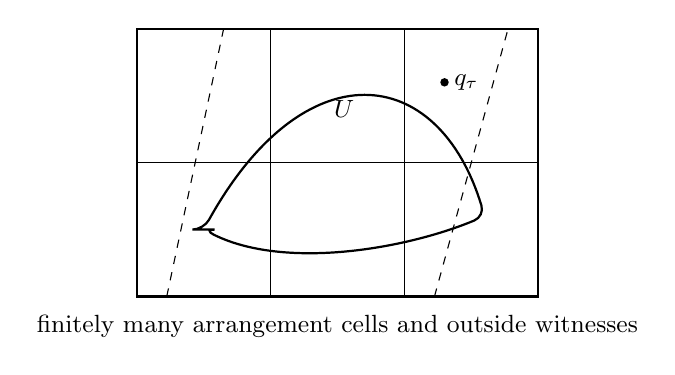
\begin{tikzpicture}[scale=.85,font=\small]
\draw[thick] (0,0) rectangle (6,4);
\draw (2,0)--(2,4); \draw (4,0)--(4,4); \draw (0,2)--(6,2);
\draw[thick,rounded corners] (1,1) .. controls (2.5,3.7) and (4.5,3.5) .. (5.2,1.2) .. controls (4,0.7) and (2.2,0.4) .. cycle;
\node at (3.1,2.8) {$U$};
\fill (4.6,3.2) circle (1.8pt) node[right]{$q_\tau$};
\draw[dashed] (4.45,0)--(5.55,4);
\draw[dashed] (0.45,0)--(1.3,4);
\node[align=center] at (3,-.45) {finitely many arrangement cells and outside witnesses};
\end{tikzpicture}